% NOTES:
% enum slide
% difference between := and =
% link and plink pic
% filter pic
% examples of running chisel

\documentclass[xcolor=pdflatex,dvipsnames,table]{beamer}
\usepackage{epsfig,graphicx}
\usepackage{palatino}
\usepackage{fancybox}
\usepackage{relsize}
\usepackage[procnames]{listings}

% "define" Scala
\usepackage[T1]{fontenc}  
\usepackage[scaled=0.82]{beramono}  
\usepackage{microtype} 

\sbox0{\small\ttfamily A}
\edef\mybasewidth{\the\wd0 }

\lstdefinelanguage{scala}{
  morekeywords={abstract,case,catch,class,def,%
    do,else,extends,false,final,finally,%
    for,if,implicit,import,match,mixin,%
    new,null,object,override,package,%
    private,protected,requires,return,sealed,%
    super,this,throw,trait,true,try,%
    type,val,var,while,with,yield},
  otherkeywords={=>,<-,<\%,<:,>:,\#,@},
  sensitive=true,
  morecomment=[l]{//},
  morecomment=[n]{/*}{*/},
  morestring=[b]",
  morestring=[b]',
  morestring=[b]"""
}

\usepackage{color}
\definecolor{dkgreen}{rgb}{0,0.6,0}
\definecolor{gray}{rgb}{0.5,0.5,0.5}
\definecolor{mauve}{rgb}{0.58,0,0.82}
 
% Default settings for code listings
\lstset{frame=tb,
  language=scala,
  aboveskip=3mm,
  belowskip=3mm,
  showstringspaces=false,
  columns=fixed, % basewidth=\mybasewidth,
  basicstyle={\small\ttfamily},
  numbers=none,
  numberstyle=\footnotesize\color{gray},
  % identifierstyle=\color{red},
  keywordstyle=\color{blue},
  commentstyle=\color{dkgreen},
  stringstyle=\color{mauve},
  frame=single,
  breaklines=true,
  breakatwhitespace=true,
  procnamekeys={def, val, var, class, trait, object, extends},
  procnamestyle=\ttfamily\color{red},
  tabsize=2
}

\lstnewenvironment{scala}
{\lstset{language=scala}}
{}
\lstnewenvironment{cpp}
{\lstset{language=C++}}
{}
\lstnewenvironment{bash}
{\lstset{language=bash}}
{}


\lstset{basicstyle={\footnotesize\ttfamily}}

\usetheme[height=8mm]{Rochester}
\setbeamersize{text margin left=3mm} 
\setbeamersize{text margin right=3mm} 
\setbeamertemplate{navigation symbols}{}

\definecolor{Cobalt}{rgb}{0.25,0.125,0.70}
\definecolor{RedOrange}{rgb}{0.8,0.25,0.0}
% \definecolor{RedOrange}{rgb}{0.8,0.775,0.25}
\def\frametitledefaultcolor{Cobalt}
\def\frametitleproblemcolor{RedOrange}

\lstset{basicstyle={\footnotesize\ttfamily}}

\setbeamertemplate{frametitle}
{
\vskip-7mm
\textbf{\insertframetitle}\hfill\insertframenumber
}
\setbeamercolor{frametitle}{bg=\frametitledefaultcolor}

\newenvironment{sample}{\VerbatimEnvironment\begin{footnotesize}\begin{semiverbatim}}{\end{semiverbatim}\end{footnotesize}}

\newenvironment{FramedSemiVerb}%
{\begin{Sbox}\begin{minipage}{.94\textwidth}\begin{semiverbatim}}%
{\end{semiverbatim}\end{minipage}\end{Sbox}
\setlength{\fboxsep}{8pt}\fbox{\TheSbox}}

\newenvironment{FramedVerb}%
{\VerbatimEnvironment
\begin{Sbox}\begin{minipage}{.94\textwidth}\begin{Verbatim}}%
{\end{Verbatim}\end{minipage}\end{Sbox}
\setlength{\fboxsep}{8pt}\fbox{\TheSbox}}

% \newenvironment{sample}{\VerbatimEnvironment\begin{footnotesize}\begin{Verbatim}}{\end{Verbatim}\end{footnotesize}}
\newcommand{\code}[1]{\begin{footnotesize}{\tt #1}\end{footnotesize}}
\newcommand{\comment}[1]{{\color{Green}\it\smaller #1}}


\title{Chisel @ CS250 -- Part II -- Lecture 03}
\author{Jonathan Bachrach}
\date{\today}
\institute[UC Berkeley]{EECS UC Berkeley}

\begin{document}

\begin{frame}
\titlepage
\end{frame}
\addtocounter{framenumber}{-1}

% \begin{frame}[fragile]{Forward Declarations using Wires}
% 
% \begin{scala}
% val pcPlus4      = UFix() 
% val branchTarget = UFix()
% val pcNext       = Mux(pcSel, branchTarget, pcPlus4)
% val pcReg        = Reg(data = pcNext, resetVal = UFix(0, 32)) 
% pcPlus4         := pcReg + UFix(4) 
% ... 
% branchTarget    := addOut
% \end{scala}
% 
% \begin{center}
% 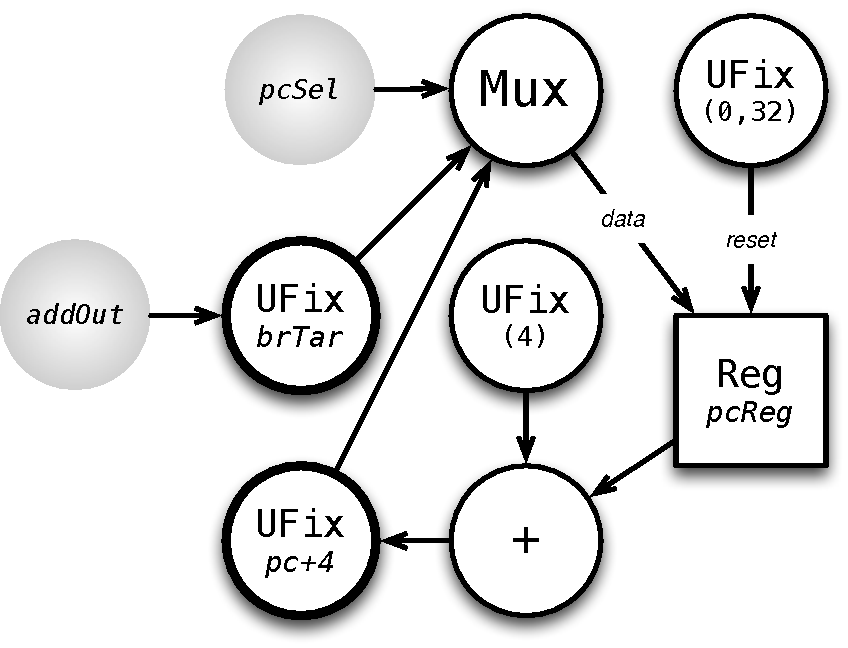
\includegraphics[height=0.5\textheight]{figs/forward.pdf} 
% \end{center}
% 
% \end{frame}

\begin{frame}[fragile]{What is Chisel?}
\begin{itemize}
\item Chisel is just a set of class definitions in Scala and
 when you write a Chisel program you are actually writing a Scala program,
\item Chisel programs produce and manipulate a data structure in Scala using a convenient textural language layered on top of Scala,
\item Chisel makes it possible to create powerful and reusable hardware components using modern programming language concepts, and
\item the same Chisel description can generate different types of output
\end{itemize}
\end{frame}

\begin{frame}[fragile]{Today}
\begin{itemize}
\item finish out state operations,
\item present how to make hierarchical components, 
\item teach you how to make reusable components,
\item introduce you to even more powerful construction techniques.
\end{itemize}
\end{frame}

\begin{frame}[fragile]{Conditional Updates}

When describing state operations, we could simply wire register inputs to combinational logic blocks, but it is often more convenient:
\begin{itemize}
\item to specify when updates to registers will occur and
\item to specify these updates spread across several separate statements
\end{itemize}

\begin{columns}
\column{0.45\textwidth}
\begin{scala}
val r = Reg() { UFix(16) }
when (c === UFix(0) ) {
  r := r + UFix(1)
}
\end{scala}

\column{0.45\textwidth}

\begin{center}
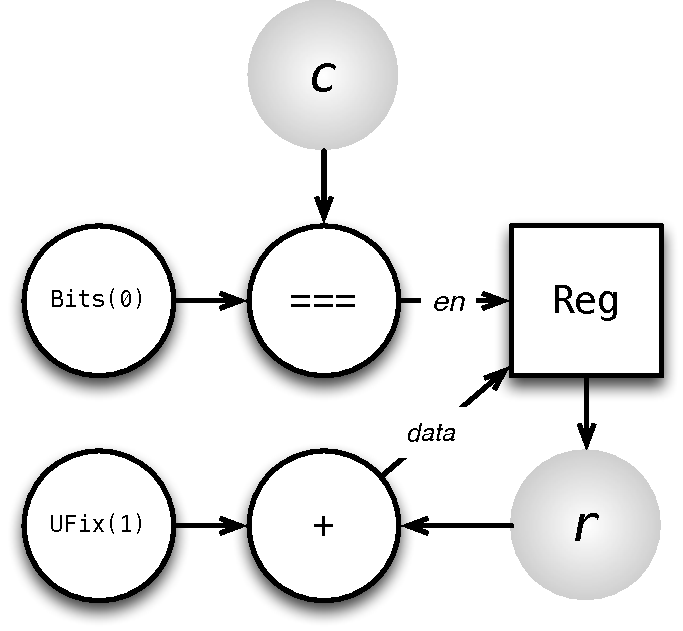
\includegraphics[width=0.9\textwidth]{figs/conditional-increment.pdf} 
\end{center}

\end{columns}
\end{frame}

\begin{frame}[fragile]{Conditional Updates Priority}

\begin{scala}
when (c1) { r := Bits(1) }
when (c2) { r := Bits(2) }
\end{scala}

\textbf{Conditional Update Order:}

\begin{center}
\begin{tabular}{|c|c|c|l|}
\hline
\code{c1} & \code{c2}  &  \code{r} & \\
\hline
0 &  0 & r &  \code{r} unchanged \\
0 &  1 & 2 & \\
1 &  0 & 1 & \\
1 &  1 & 2 & \code{c2} takes precedence over \code{c1} \\
\hline
\end{tabular}
\end{center}

\end{frame}

\begin{frame}[fragile]{Conditional Update Synthesized Hardware}

\begin{center}
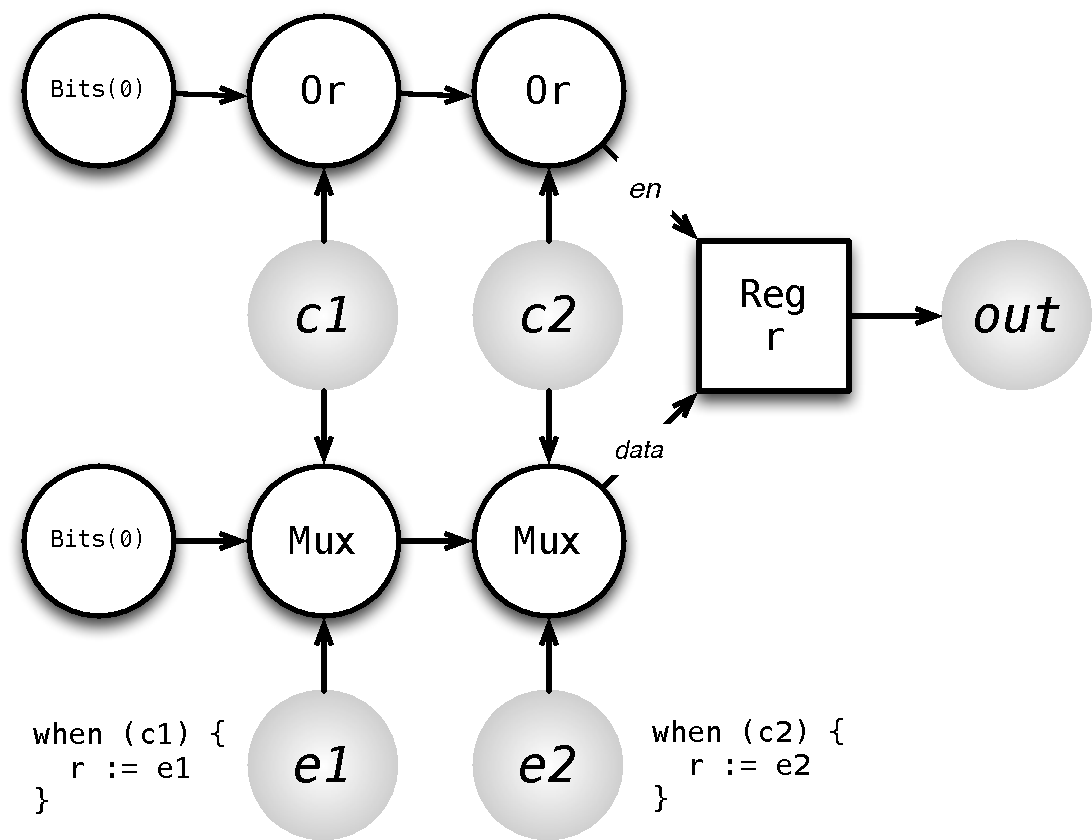
\includegraphics[height=2in]{figs/conditional-updates.pdf}
\end{center}

\begin{itemize}
\item Each \code{when} statement adds another level of data mux and ORs
  the predicate into the enable chain and
\item the compiler effectively adds
  the termination values to the end of the chain automatically.
\end{itemize}

\end{frame}

\begin{frame}[fragile]{Targetting Multiple Registers}

\begin{scala}
r := Reg(){ Fix(3) }
s := Reg(){ Fix(3) }
when (c1) { r := Fix(1); s := Fix(1) }
when (c2) { r := Fix(2) }
\end{scala}

leads to \code{r} and \code{s} being updated according to the
following truth table:

{\footnotesize
\begin{center}
\begin{tabular}{|c|c|c|c|l|}
\hline
\code{c1} & \code{c2}  & \code{r} & \code{s} & \\
\hline 
0 &  0 & 3 & 3 & \\
0 &  1 & 2 & 3 & \\ 
1 &  0 & 1 & 1 & \code{r} updated in \code{c2} block, \code{s} updated using default \\
1 &  1 & 2 & 1 & \\
\hline
\end{tabular}
\end{center}
}

\end{frame}

\begin{frame}[fragile]{Conditional Update Nesting}

\begin{scala}
when (a) { when (b) { body } }
\end{scala}

which is the same as:

\begin{scala}
when (a && b) { body }
\end{scala}

\end{frame}

\begin{frame}[fragile]{Conditional Update Chaining}

\begin{scala}
when (c1) { u1 }
.elsewhen (c2) { u2 }
.otherwise { ud }
\end{scala}

which is the same as:

\begin{scala}
when (c1) { u1 }
when (!c1 && c2) { u2 }
when (!(c1 || c2)) { ud }
\end{scala}

\end{frame}

\begin{frame}[fragile]{Switch Statement}

\begin{scala}
switch(idx) {
  is(v1) { u1 }
  is(v2) { u2 }
}
\end{scala}

which is the same as:

\begin{scala}
when (idx === v1) { u1 }
when (idx === v2) { u2 }
\end{scala}

\end{frame}

% \begin{frame}[fragile]{Enums}
% \begin{scala}
% val s_even :: s_odd :: Nil = Enum(2){ UFix() }
% \end{scala}
% \end{frame}


\begin{frame}[fragile]{Conditional Updates Everywhere}
Conditional updates also work for 
\begin{itemize}
\item wires but must have defaults and
\item for memory reads and writes as we'll see soon...
\end{itemize}

For wires, we can do conditional updates as follows:

\begin{scala}
val w = Bits(width = 32)
w := Bits(0)                       // default value 
when (c1)         { w := Bits(1) }
when (c2)         { w := Bits(2) }
\end{scala}

\noindent
which is the same as

\begin{scala}
val w = Bits(width = 32)
when (Bool(true)) { w := Bits(0) } // default value
when (c1)         { w := Bits(1) }
when (c2)         { w := Bits(2) }
\end{scala}

\end{frame}

\begin{frame}[fragile]{Finite State Machines}

\begin{columns}
\column{0.65\textwidth}

Finite state machines can now be readily defined as follows:

\begin{scala}
class Parity extends Component {
  val io = new Bundle {
    val in  = Bool(INPUT)
    val out = Bool(OUTPUT) }
  val s_even :: s_odd :: Nil = Enum(2){ UFix() }
  val state  = Reg(resetVal = s_even)
  when (io.in) {
    when (state === s_even) { state := s_odd  }
    .otherwise              { state := s_even }
  }
  io.out := (state === s_odd)
}
\end{scala}

\noindent
where \verb+Enum(2){ UFix() }+ creates a list of two \code{UFix()} literals.
\column{0.25\textwidth}

\begin{center}
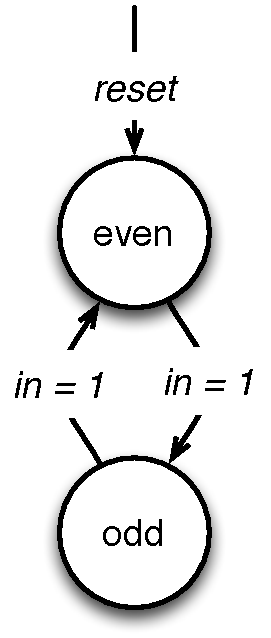
\includegraphics[height=0.9\textheight]{figs/parity.pdf} 
\end{center}

\end{columns}
\end{frame}

\begin{frame}[fragile]{ROM}

\begin{scala}
val d = Array(UFix(1), UFix(2), UFix(4), UFix(8))
val m = ROM(d){ UFix(width = 32) }
val r = m(counter(UFix(3)))
\end{scala}

\begin{center}
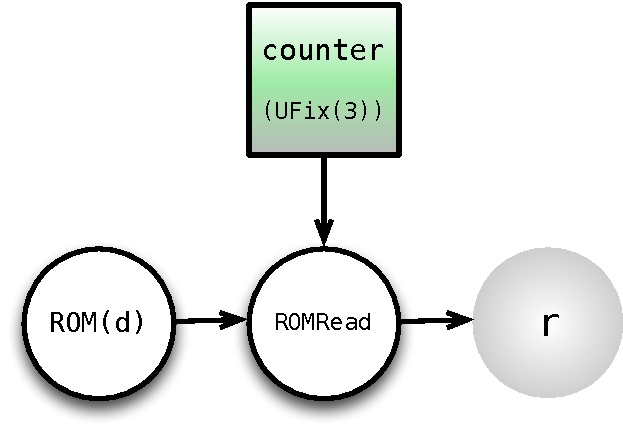
\includegraphics[height=0.7\textheight]{figs/rom.pdf} 
\end{center}

\end{frame}

\begin{frame}[fragile]{Mul Lookup Table}
\begin{columns}
\column{0.52\textwidth}

\begin{scala}
class Mul extends Component {
  val io = new Bundle {
    val x   = UFix(INPUT, 4)
    val y   = UFix(INPUT, 4)
    val z   = UFix(OUTPUT, 8) }

  val muls = new Array[UFix](256)
  for (x <- 0 until 16; y <- 0 until 16) 
    muls((x << 4) | y) = x * y

  val tbl = ROM(muls){ UFix(8) }

  io.z := tbl((io.x << 4) | io.y)
}
\end{scala}

\column{0.38\textwidth}

\begin{center}
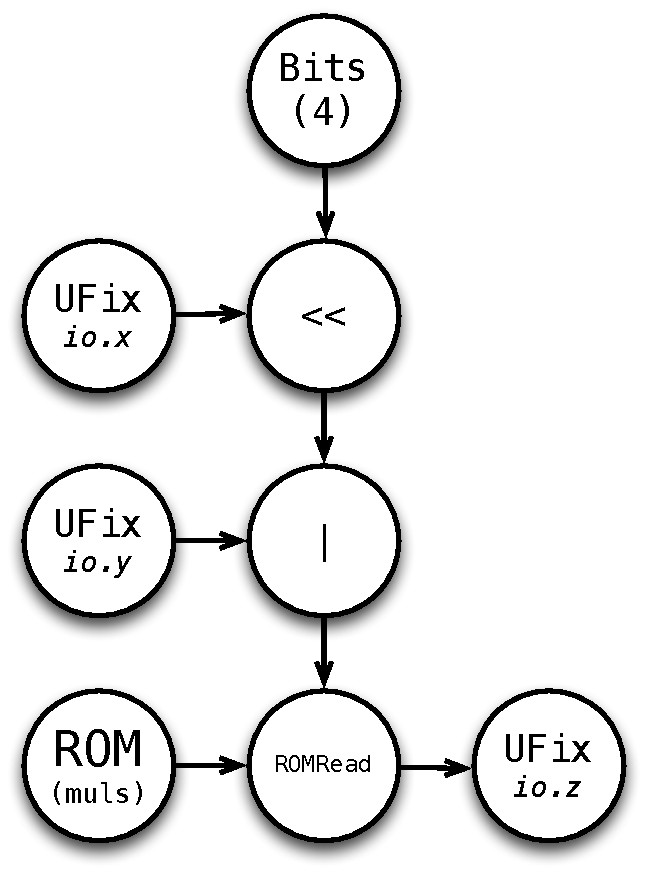
\includegraphics[width=0.9\textwidth]{figs/muls.pdf} 
\end{center}

\end{columns}
\end{frame}

\begin{frame}[fragile]{RAM}

RAM is supported using the \code{Mem} construct

\begin{scala}
val m = Mem(32){ Bits(width = 32) }
\end{scala}

\noindent
where
\begin{itemize}
\item writes to Mems are positive-edge-triggered
\item reads are either combinational or positive-edge-triggered
\item ports are created by applying a \code{UFix} index
\end{itemize}
\end{frame}

\begin{frame}[fragile]{32-entry Register File}

\begin{scala}
val regs = Mem(32){ Bits(width = 32) }
when (wrEn) {
  regs(wrAddr) := wrData
}
val iDat = regs(iAddr)
val mDat = regs(mAddr)
\end{scala}

\begin{center}
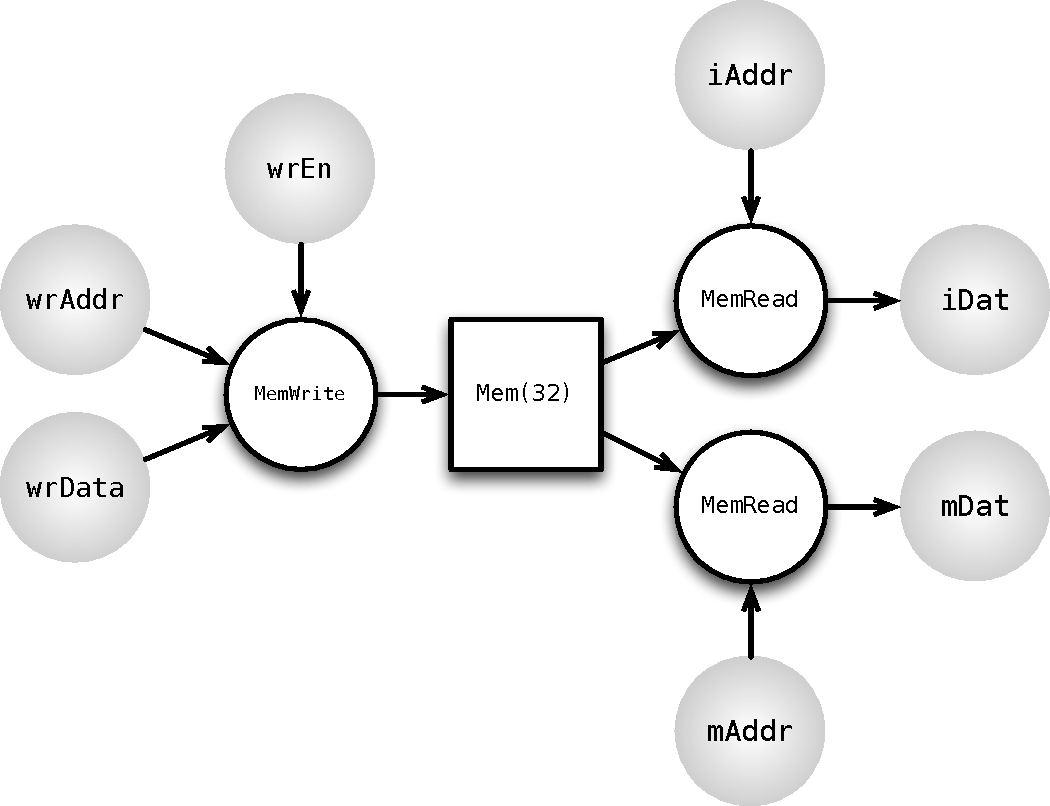
\includegraphics[height=0.55\textheight]{figs/mem.pdf} 
\end{center}

\end{frame}

\begin{frame}[fragile]{Sequential Read Ports}

Sequential read ports are inferred when:
\begin{itemize}
\item optional parameter \code{seqRead} is set and
\item a reg is assigned to the output of a MemRead
\end{itemize}

\begin{scala}
val ram1r1w = Mem(1024, seqRead = true) { Bits(width = 32) }
val dOut    = Reg() { Bits() }
when (wrEn) { ram1r1w(wrAddr) := wrData }
when (rdEn) { dOut := ram1r1w(rdAddr) }
\end{scala}

\begin{center}
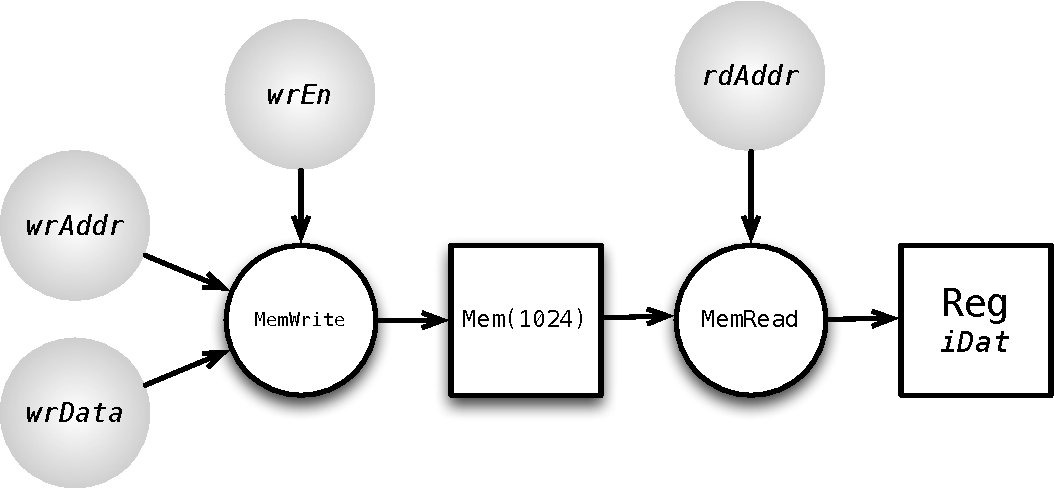
\includegraphics[height=0.4\textheight]{figs/mem-seq-read.pdf} 
\end{center}

\end{frame}

\begin{frame}[fragile]{Single-ported SRAM}

Single-ported SRAMs can be inferred when the read and write conditions are
mutually exclusive in the same \code{when} chain

\begin{scala}
val ram1p = Mem(1024, seqRead = true) { Bits(width = 32) }
val dOut  = Reg() { Bits() }
when (wrEn) { ram1p(wrAddr) := wrData }
.elsewhen (rdEn) { dOut := ram1p(rdAddr) }
\end{scala}

\begin{center}
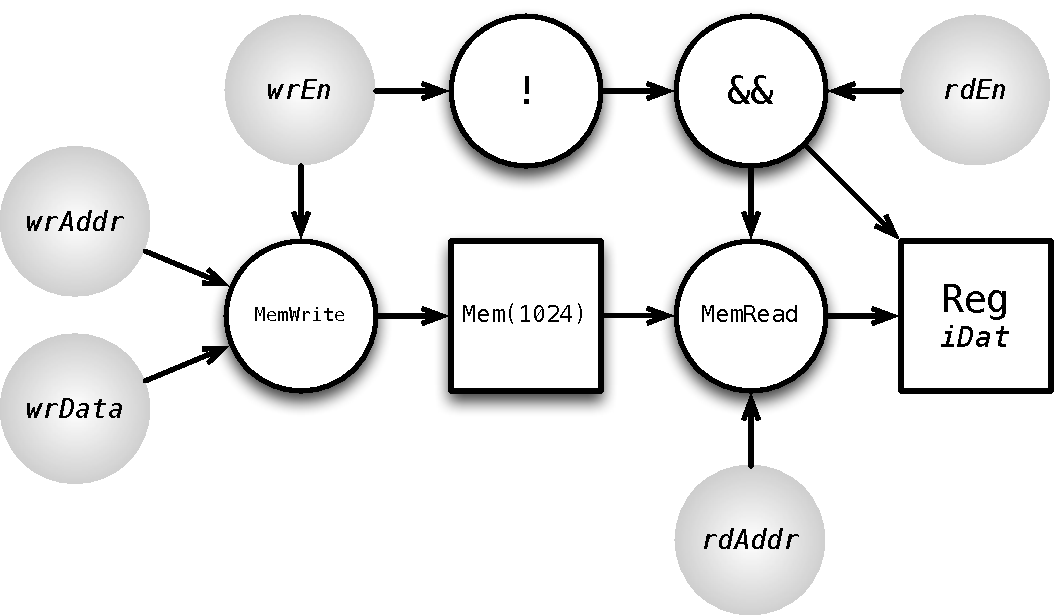
\includegraphics[height=0.5\textheight]{figs/mem-single-ported.pdf} 
\end{center}

\end{frame}

\begin{frame}[fragile]{Components and Interfaces}

Suppose we want to break computation into a series of filters (ala Unix):

\begin{center}
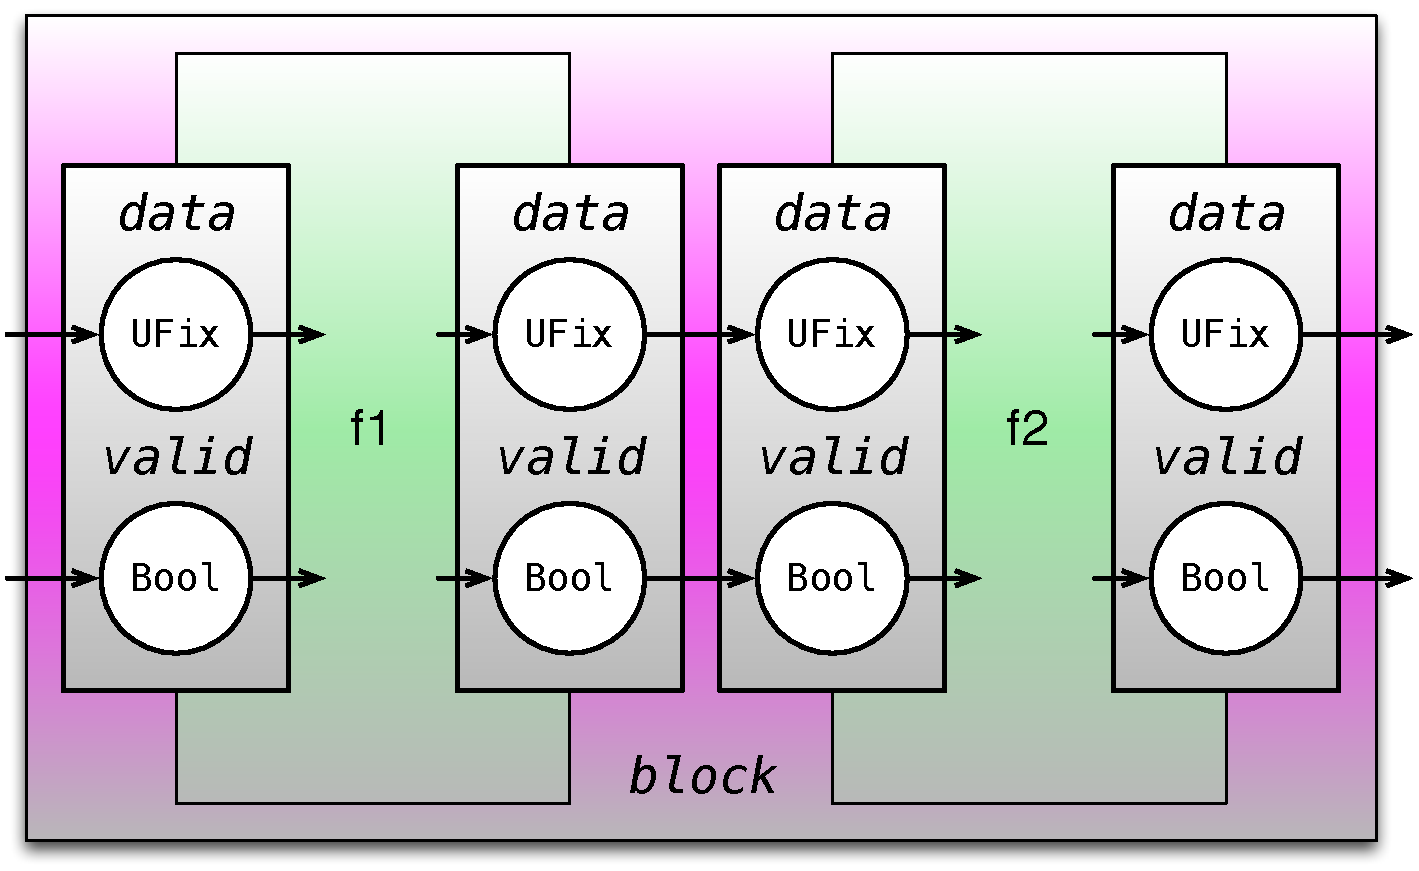
\includegraphics[width=0.7\textwidth]{figs/filtering.pdf} 
\end{center}

\noindent 
where data is fed though with an additional \code{valid} signal to say whether data has \textbf{not} been filtered.

\end{frame}

\begin{frame}[fragile]{Pass Through Filter}

We can define a pass through filter component by defining a filter class extending component:

\begin{columns}
\column{0.45\textwidth}

\begin{scala}
class Filter extends Component { 
  val io  = new FilterIO()
  io.out.data  := io.in.data
  io.out.valid := io.in.valid
}
\end{scala}

\column{0.45\textwidth}

\begin{center}
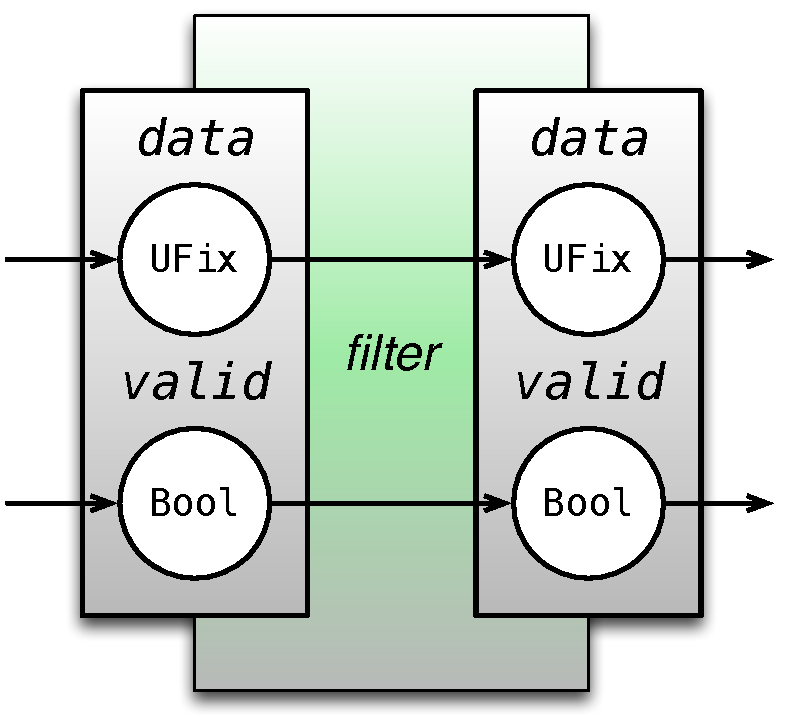
\includegraphics[width=0.9\textwidth]{figs/pass-through-filter.pdf} 
\end{center}
\end{columns}

\noindent 
where the \verb+io+ field contains \verb+FilterIO+. 
\end{frame}

\begin{frame}[fragile]{Small and Odd Filters}

Suppose we want to write a small and odd filter.  We could write these out by hand:

\begin{scala}
class SmallFilter extends Component { 
  val io  = new FilterIO()
  io.out.data  := io.in.data
  io.out.valid := io.in.valid && (io.in.data < 10)
}

class OddFilter extends Component { 
  val io  = new FilterIO()
  io.out.data  := io.in.data
  io.out.valid := io.in.valid && (io.in.data & 1)
}
\end{scala}

\end{frame}

\begin{frame}[fragile]{Basic Filter Interface}

\begin{columns}
\column{0.55\textwidth}

\begin{scala}
class PipeIO extends Bundle { 
  val data  = UFix(OUTPUT, 16) 
  val valid = Bool(OUTPUT)
}
\end{scala}

\column{0.35\textwidth}

\begin{center}
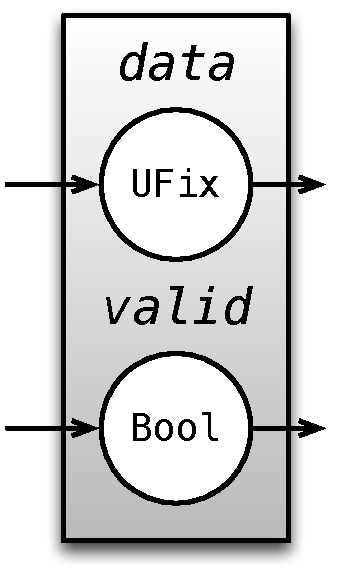
\includegraphics[height=0.9\textheight]{figs/link-io.pdf} 
\end{center}

\end{columns}
\end{frame}

\begin{frame}[fragile]{Complete Filter Interface}

\begin{columns}
\column{0.55\textwidth}

From there we can define a filter interface by nesting two
\verb+PipeIO+s into a new \verb+FilterIO+ bundle:

\begin{scala}
class FilterIO extends Bundle { 
  val in  = new PipeIO().flip
  val out = new PipeIO()
}
\end{scala}

\noindent
where \verb+flip+ recursively changes the ``gender'' of a bundle,
changing input to output and output to input.

\column{0.35\textwidth}

\begin{center}
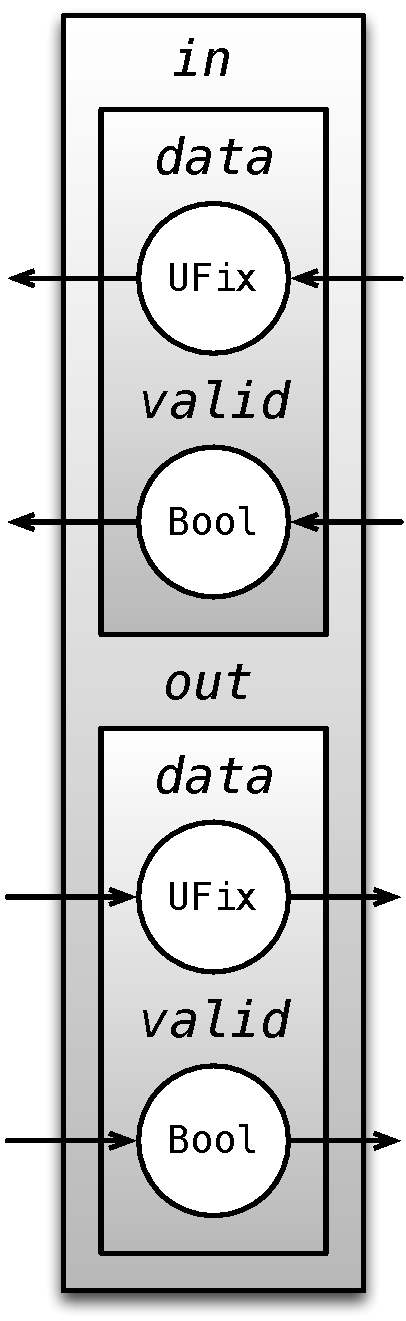
\includegraphics[height=0.9\textheight]{figs/filter-io.pdf} 
\end{center}

\end{columns}
\end{frame}

\begin{frame}[fragile]{Bulk Connections}
We can now compose two filters into a filter block as follows:

\begin{columns}
\column{0.42\textwidth}

{\lstset{basicstyle={\scriptsize\ttfamily}}
\begin{scala}
class SmallOdds extends Component { 
  val io     = new FilterIO()
  val smalls = new SmallFilter()
  val odds   = new OddFilter()

  smalls.io.in  <> io.in
  smalls.io.out <> odds.io.in
  odds.io.out   <> io.out
}
\end{scala}
}

\column{0.48\textwidth}

\begin{center}
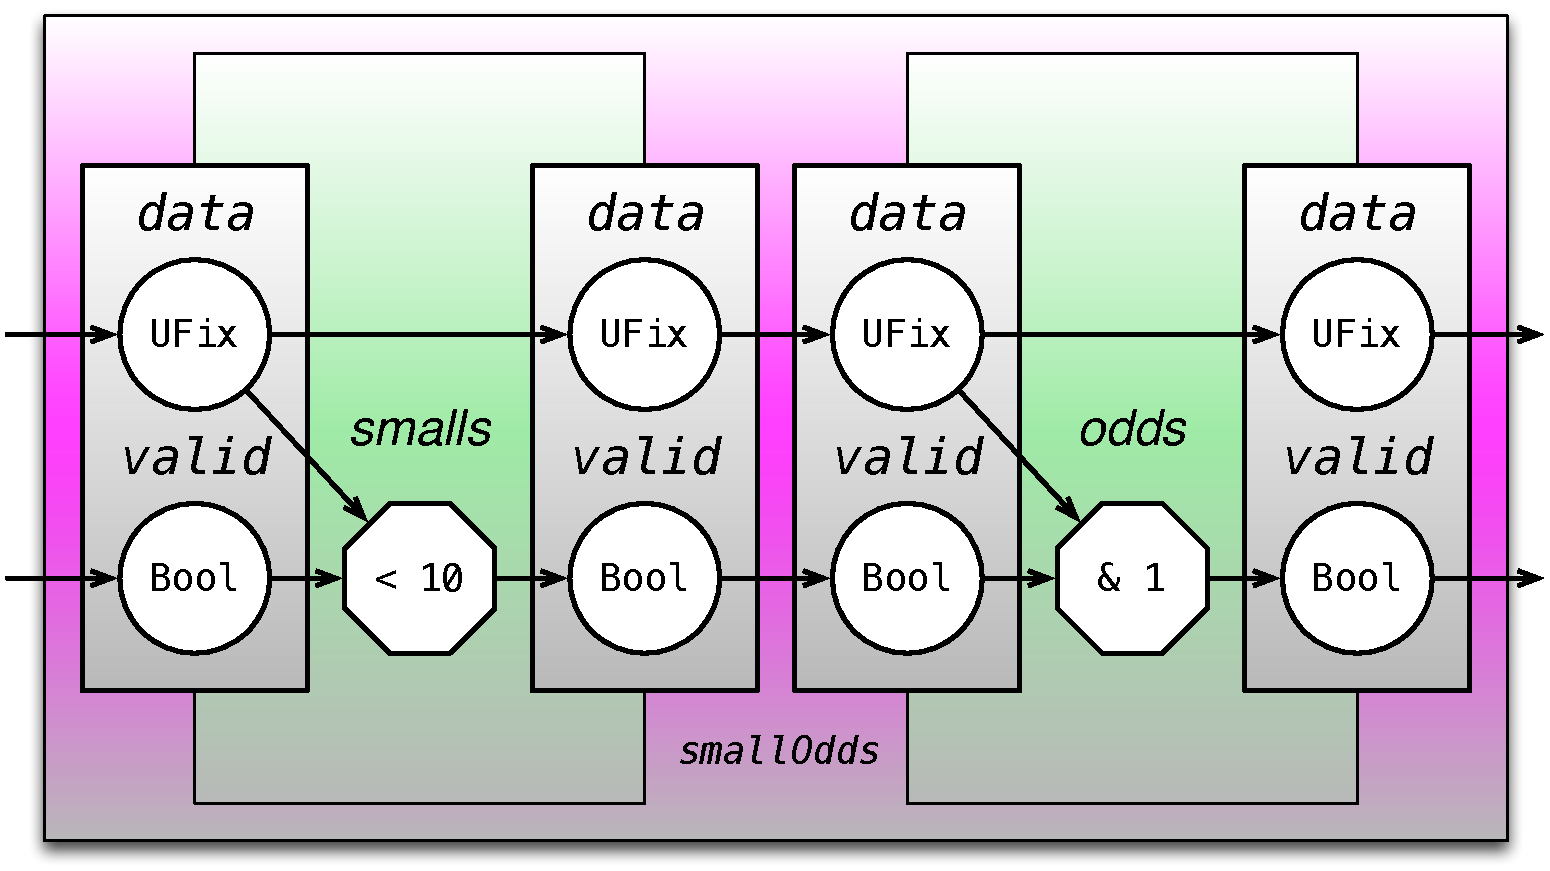
\includegraphics[width=0.95\textwidth]{figs/small-odds.pdf} 
\end{center}

\end{columns}

\noindent
where \verb+<>+ bulk connects interfaces.  Note that:
\begin{itemize}
\item bulk connections recursively pattern match names between left and right hand sides finally connecting leaf ports to each other, and
\item after all connections are made and the circuit is being elaborated,
Chisel warns users if ports have other than exactly one connection to them.
\end{itemize}
\end{frame}

\begin{frame}{Prepare for Warp Speed and Be Happy}

Congratulations, you have all that you need at this point to write Chisel programs!
You can write RTL, define components (even with recursive data types), and wire them together.
\vspace{5mm}
\begin{itemize}
\item In order to attain true hardware description power though, you need to be able to write reusable RTL, components and interfaces.
\item This will allow you to both use and write generic component libraries and more quickly explore design space.
\item To do this, we will use modern programming techniques such as:
\begin{itemize}
\item object orientation, 
\item functional programming, 
\item parameterized types
\end{itemize}
\item You will be greatly rewarded for your efforts!
\end{itemize}

\end{frame}


\begin{frame}[fragile]{Parameterized Filter}

Instead of writing a \code{SmallFilter} and \code{OddFilter}, a better Filter solution would be to create a single reusable Filter class that allows the user to specify the filter function.  We can do this by
\begin{itemize}
\item specifying a filter function as a Filter constructor argument:
\end{itemize}

\begin{columns}
\column{0.55\textwidth}

{\lstset{basicstyle={\scriptsize\ttfamily}}
\begin{scala}
class Filter (isOk: (UFix) => Bool) 
    extends Component { 
  val io  = new FilterIO()
  io.out.data  := io.in.data
  io.out.valid := 
    io.in.valid && isOk(io.in.data)
}

val odds   = new Filter((x) => x & UFix(1))
val smalls = new Filter((x) => x < UFix(10))
\end{scala}
}

\column{0.40\textwidth}

\begin{center}
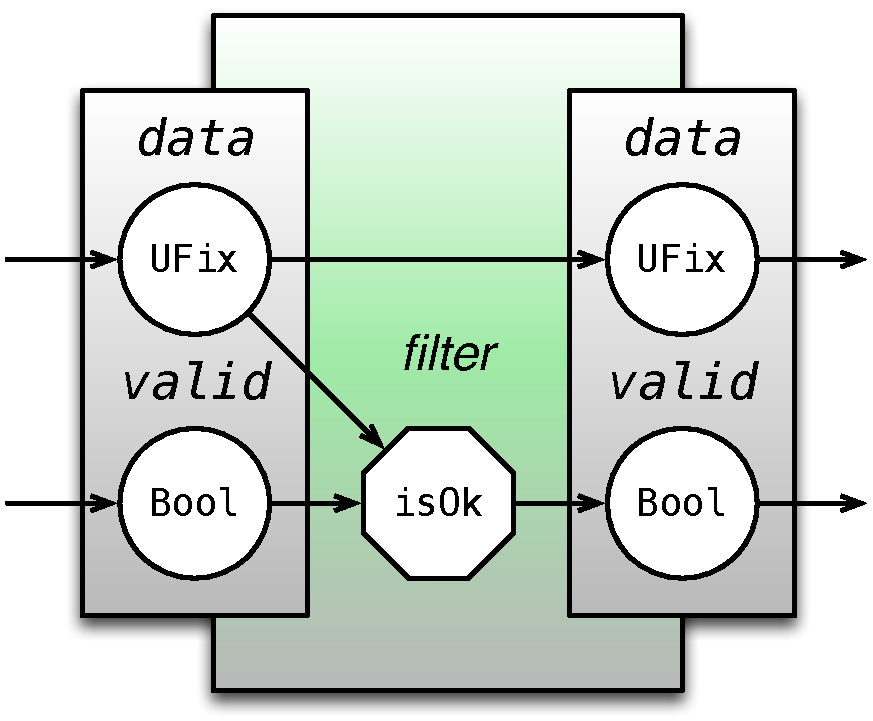
\includegraphics[width=0.9\textwidth]{figs/parameterized-filter.pdf} 
\end{center}
\end{columns}

\end{frame}

\begin{frame}[fragile]{SmallOdds built out of Parameterized Filters}
We can now compose two parameterized filters into a filter block as follows:

\begin{columns}
\column{0.42\textwidth}

{\lstset{basicstyle={\scriptsize\ttfamily}}
\begin{scala}
class SmallOdds extends Component { 
  val io     = new FilterIO()
  val smalls = new Filter(_ < 10)
  val odds   = new Filter(_ & 1)

  smalls.io.in  <> io.in
  smalls.io.out <> odds.io.in
  odds.io.out   <> io.out
}
\end{scala}
}

\column{0.48\textwidth}

\begin{center}
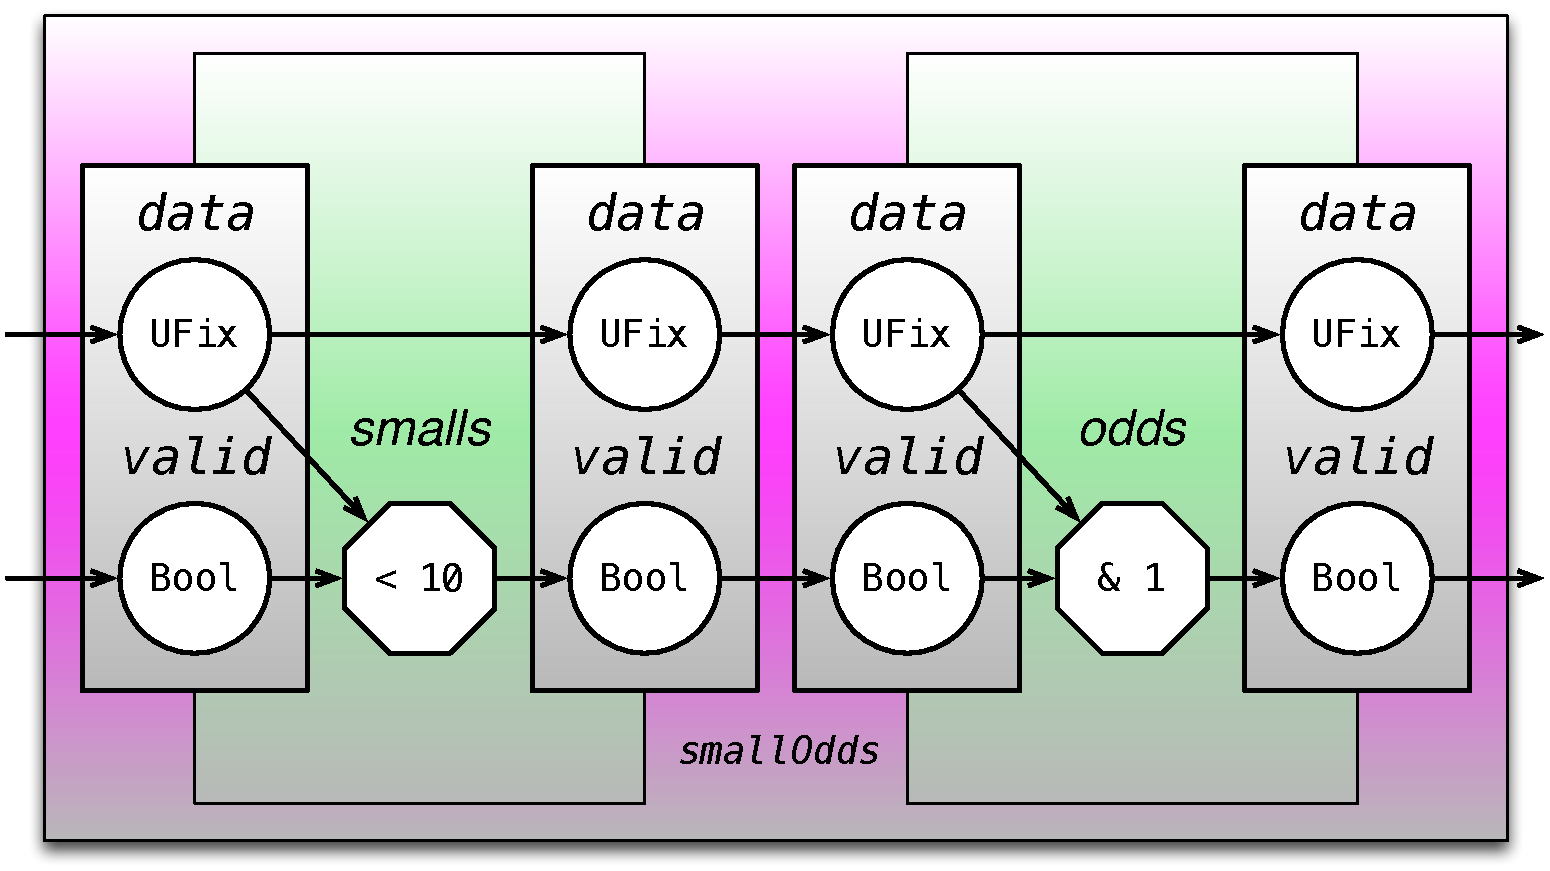
\includegraphics[width=0.95\textwidth]{figs/small-odds.pdf} 
\end{center}

\end{columns}

\noindent
where \code{\_ \& 1} is a shorthand for \code{(x) => x \& 1}.
\end{frame}

\begin{frame}[fragile]{Decoupled Filters}
Suppose we want to make a block of two filters, where the filters take differing amounts of time to compute and need to be decoupled from each other.
We can do this:
\begin{itemize}
\item by using decoupled interfaces with an additional ready signal and
\item by connecting the two filters up using a queue
\end{itemize}

\begin{columns}
\column{0.41\textwidth}

{\lstset{basicstyle={\scriptsize\ttfamily}}
\begin{scala}
class SmallOdds extends Component { 
  val io     = new FilterIO()
  val smalls = new Filter(_ < 10)
  val q      = new Queue()
  val odds   = new Filter(_ & 1)

  smalls.io.in  <> io.in
  smalls.io.out <> q.io.in
  q.io.out      <> odds.io.in
  odds.io.out   <> io.out
}
\end{scala}
}

\column{0.49\textwidth}

\begin{center}
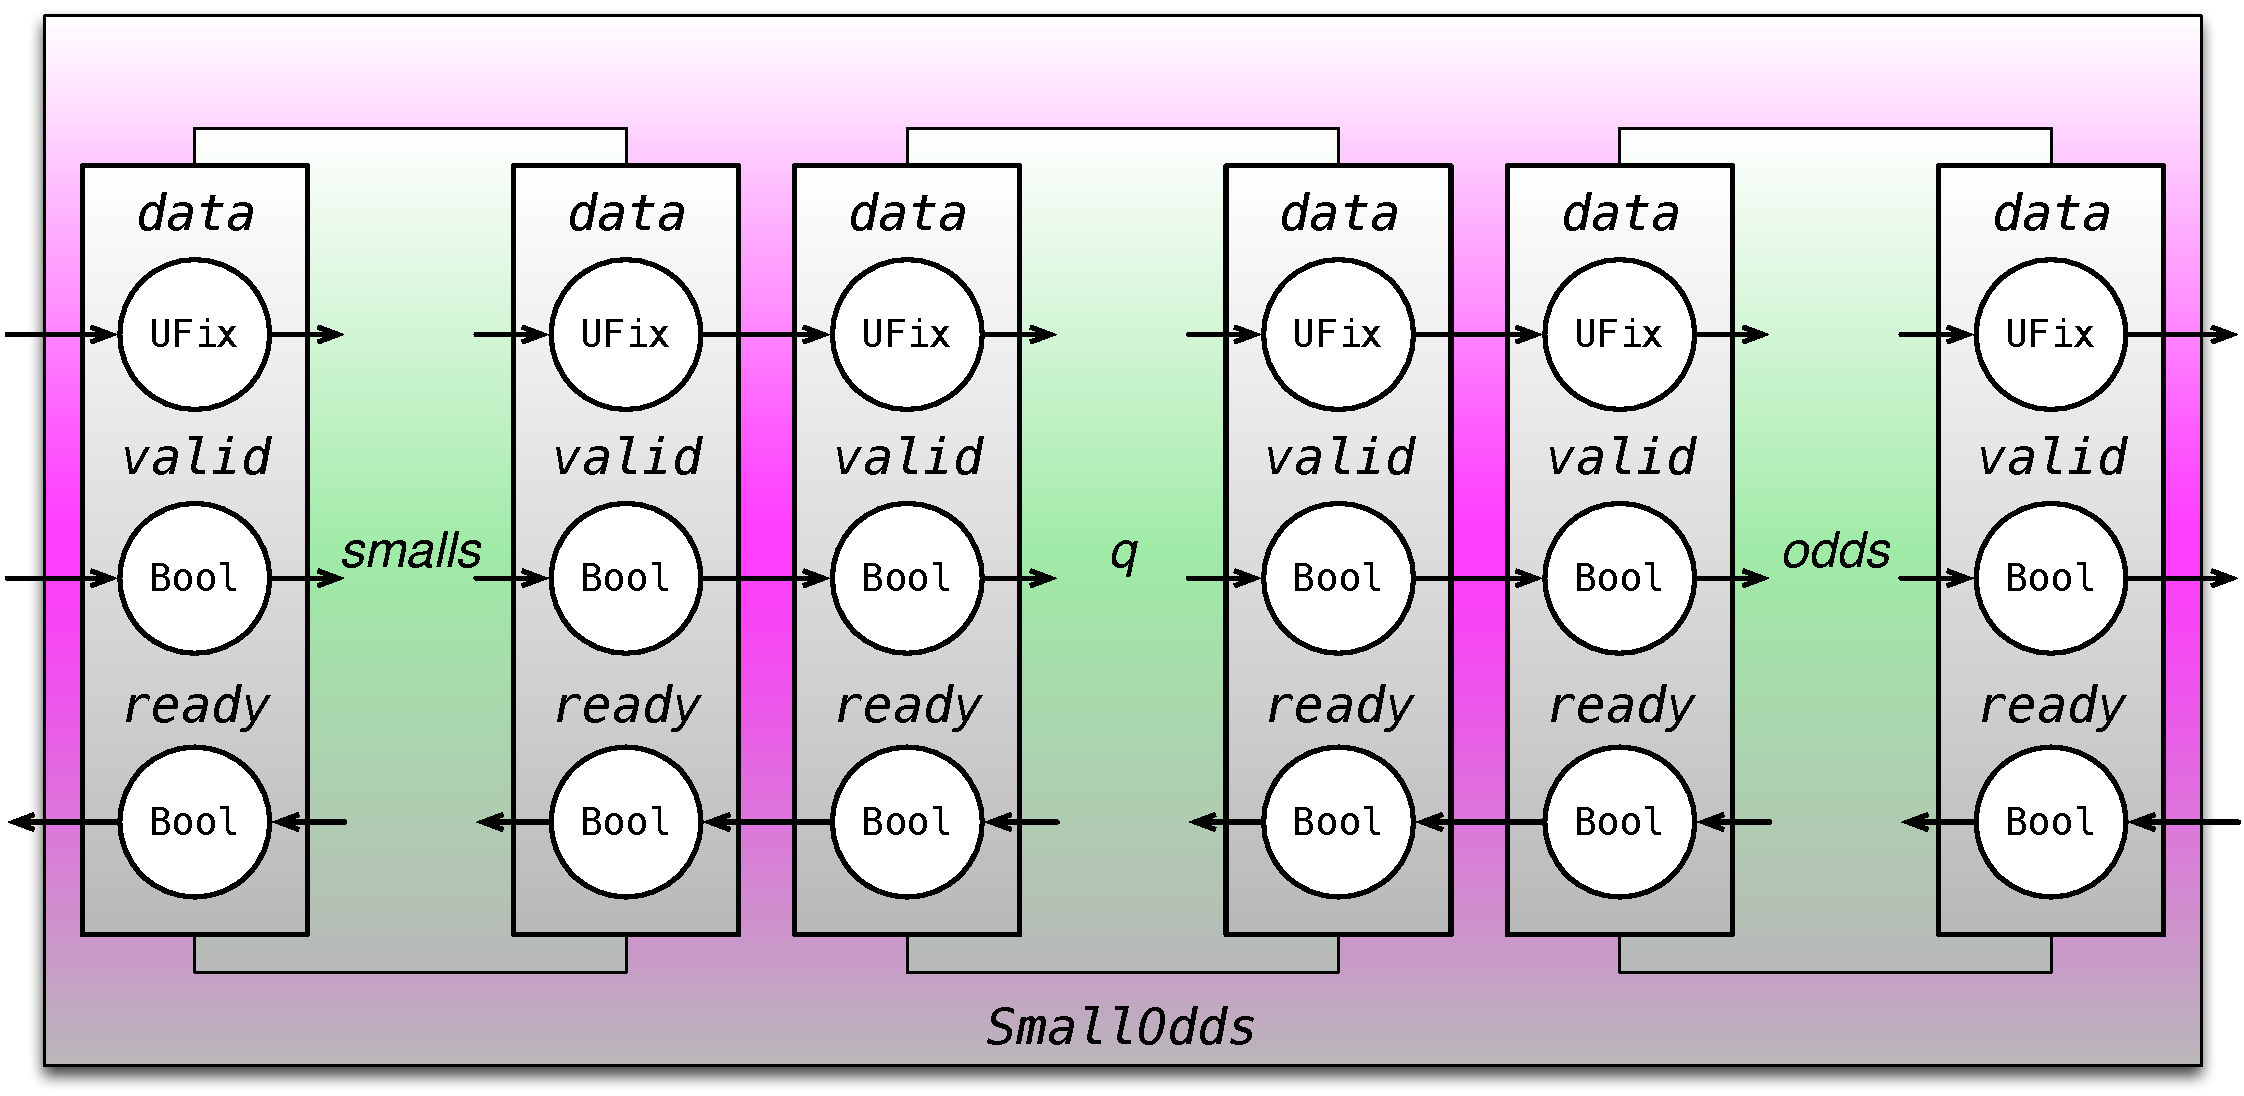
\includegraphics[width=1.0\textwidth]{figs/decoupled-block.pdf} 
\end{center}

\end{columns}

\end{frame}

\begin{frame}[fragile]{Decoupled Filter}

Now filtering must consider back pressure:

\begin{columns}
\column{0.45\textwidth}

{\lstset{basicstyle={\scriptsize\ttfamily}}
\begin{scala}
class Filter (isOk: (UFix) => Bool) 
    extends Component { 
  val io  = new FilterIO()
  io.out.data  := io.in.data
  io.out.ready := Bool(true)
  io.out.valid := 
    io.out.ready && 
    io.in.valid && 
    isOk(io.in.data)
}
\end{scala}
}

\column{0.45\textwidth}

\begin{center}
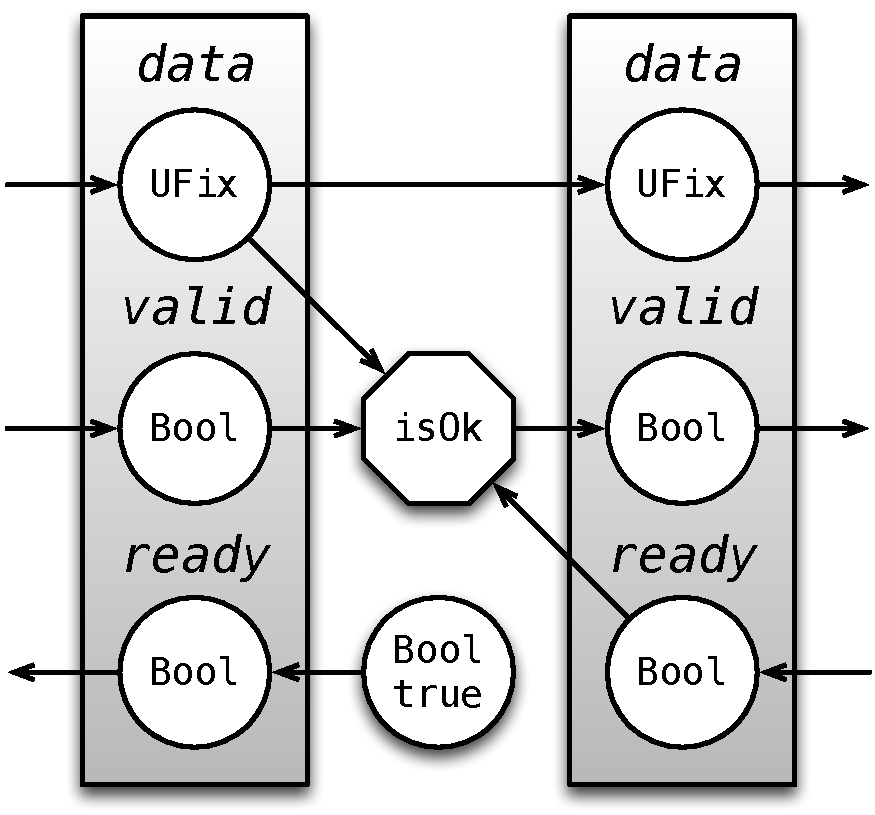
\includegraphics[width=0.9\textwidth]{figs/odd-filter.pdf} 
\end{center}
\end{columns}

\vspace{3mm}
\noindent 
where 
\begin{itemize}
\item the filter ``fires'' only when there is input data present and upstream fifos and filters are ready for output data, and
\item in this version we are assuming that we are always ready for data.
\end{itemize}

\end{frame}

\begin{frame}[fragile]{Basic Decoupled IO}

\begin{columns}
\column{0.55\textwidth}

We can define a decoupled interface by extending \verb+PipeIO+ with a ready signal:

\begin{scala}
class FIFOIO extends PipeIO { 
  val ready = Bool(INPUT)
}
\end{scala}

\noindent
In general, users can organize their interfaces into hierarchies using inheritance in order to promote reuse.  

\column{0.35\textwidth}

\begin{center}
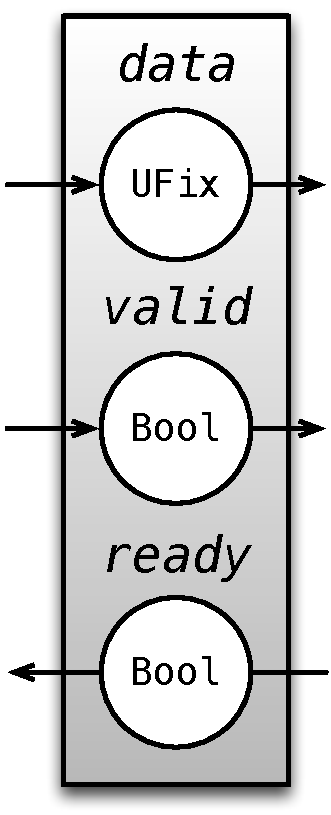
\includegraphics[height=0.9\textheight]{figs/FIFOIO.pdf} 
\end{center}

\end{columns}

\end{frame}

\begin{frame}[fragile]{Complete Decoupled Filter Interface}

\begin{columns}
\column{0.55\textwidth}

From there we can define a filter interface by nesting two
\verb+FIFOIO+s into a new \verb+FilterIO+ bundle:

\begin{scala}
class FilterIO extends Bundle { 
  val in  = new FIFOIO().flip
  val out = new FIFOIO()
}
\end{scala}

\column{0.35\textwidth}

\begin{center}
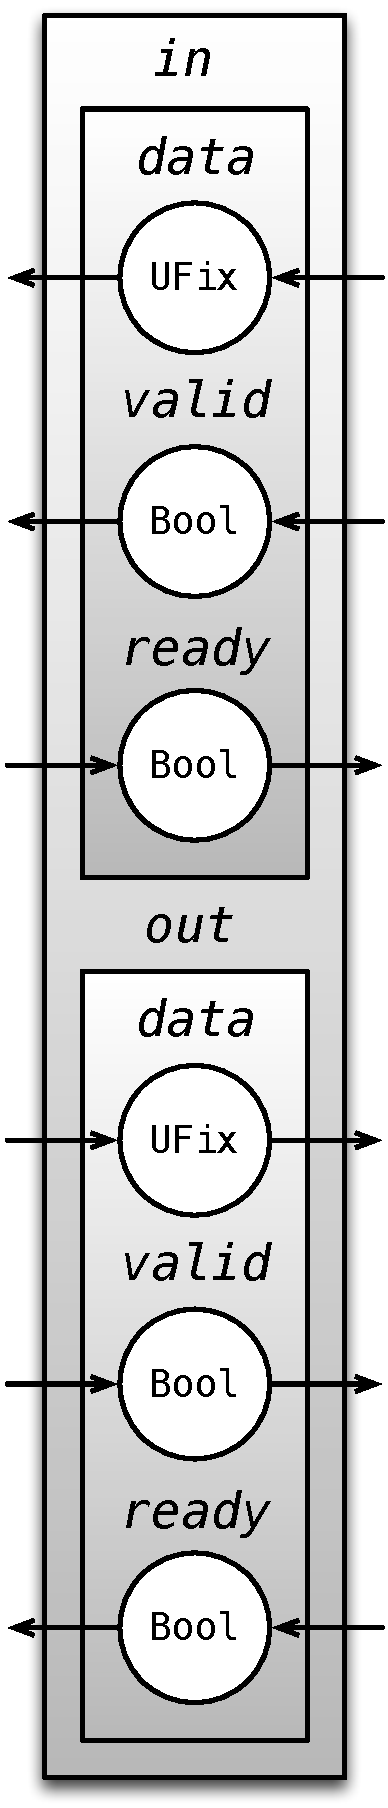
\includegraphics[height=0.9\textheight]{figs/decoupled-filter-io.pdf} 
\end{center}

\end{columns}
\end{frame}

\begin{frame}[fragile]{Parameterized Decoupled Interfaces}

Unfortunately, as defined, decoupled interfaces are defined only for 16 bit \verb+UFix+s.  
Obviously, we want to generalize this to allow for arbitrary Chisel data types.  
We can do this by using:
\begin{itemize}
\item Scala parameterized types and 
\item a curried class constructor argument
\end{itemize}

We want to be able to write
\begin{scala}
val ufix32s = new FIFOIO(){ UFix(width = 32) }

class Packet extends Bundle {
  val header = UFix(width = 8)
  val body   = Bits(width = 64)
}
val pkts    = new FIFOIO(){ new Packet() }
\end{scala}

\noindent
but how do we define this parameterized \code{FIFOIO}?
\end{frame}

\begin{frame}[fragile]{Parameterized Types in Scala}

First we need to learn about parameterized types in Scala.
We can define a generic \code{Mux} function as taking a boolean condition and \code{con} and \code{alt} arguments (corresponding to then and else expressions) of type \code{T} as follows:

\begin{scala}
def Mux[T <: Bits](c: Bool, con: T, alt: T): T { ... }
\end{scala}

\noindent
where 
\begin{itemize}
\item \code{T} is required to be a subclass of \code{Bits} and 
\item the type of \code{con} and \code{alt} are required to match.
\end{itemize}

\noindent
You can think of the type parameter as a way of just constraining the types of the allowable arguments.

\end{frame}

\begin{frame}[fragile]{Curried Arguments}

In Chisel we use special syntax for passing in a type constructor for parameterized types (such as Reg, Mem, and ROM).  For example, for we can construct a reg using the following syntax:
\begin{scala}
val r = Reg(){ Bits(width = 32) }
\end{scala}

You can write your own functions to allow this syntax and behavior as follows:

\begin{scala}
def myReg[T <: Data]()(type: => T) { ... }

myReg(){ Bits(width = 16) }
\end{scala}

\noindent
where the second parameter list has a single zero argument function parameter (aka thunk) that when called with no arguments produces a chisel type.

\end{frame}

\begin{frame}[fragile]{Implementing Parameterized Interfaces}

Now we can define \code{FIFOIO} and \code{FilterIO} using parameterized types and a curried argument as follows:

{\lstset{basicstyle={\scriptsize\ttfamily}}
\begin{scala}
class FIFOIO[T <: Data]()(type: => T) extends Bundle {
  val data  = type.asOutput
  val valid = Bool(OUTPUT)
  val ready = Bool(INPUT)
}

class FilterIO[T <: Data]()(type: => T) extends Bundle { 
  val in  = new FIFOIO(){ type }.flip
  val out = new FIFOIO(){ type }
}
\end{scala}

\noindent
We can now define \code{FIFOIO} on arbitrary data types:

\begin{scala}
val ufix32s = new FIFOIO(){ UFix(width = 32) }
val pkts    = new FIFOIO(){ new Packet() }
\end{scala}
}
\end{frame}

\begin{frame}[fragile]{Fully Parameterized Filters}

Now we can redo our definition of the \code{Filter} and \code{SmallOdds} components:

{\lstset{basicstyle={\scriptsize\ttfamily}}
\begin{scala}
class Filter[T <: Data] (isOk: (T) => Bool) (type: => T) extends Component { 
  val io = new FilterIO(){ type }

  io.out.data  := io.in.data
  io.out.ready := Bool(true)
  io.out.valid := io.out.ready && io.in.valid && isOk(io.in.data)
}

class SmallOdds[T <: Data]()(type: => T) extends Component { 
  val io     = new FilterIO()
  val smalls = new Filter(_ < UFix(10)){ type }
  val q      = new Queue(){ type }
  val odds   = new Filter(_ & UFix(1)){ type }

  smalls.io.in  <> io.in
  smalls.io.out <> q.io.in
  q.io.out      <> odds.io.in
  odds.io.out   <> io.out
}

val block = new SmallOdds(){ UFix(width = 32) }
\end{scala}
}
\end{frame}

\begin{frame}[fragile]{Interface Views}
\begin{columns}
\column{0.40\textwidth}

\begin{scala}
class Cpu extends Component {
  val io = new CpuIo()
  val c  = new CtlPath()
  val d  = new DatPath()
  c.io.ctl  <> d.io.ctl
  c.io.dat  <> d.io.dat
  c.io.imem <> io.imem
  d.io.imem <> io.imem
  c.io.dmem <> io.dmem
  d.io.dmem <> io.dmem
  d.io.host <> io.host
}
\end{scala}

\column{0.50\textwidth}

\begin{center}
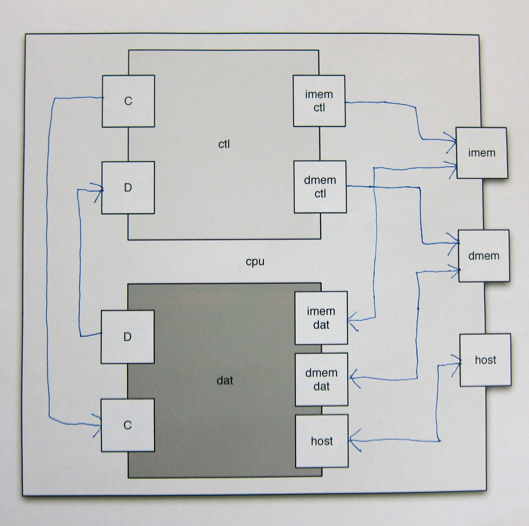
\includegraphics[width=0.9\textwidth]{../tutorial/figs/cpu.png} 
\end{center}

\end{columns}
\end{frame}

\begin{frame}[fragile]{CPU Interfaces}
\begin{columns}
\column{0.40\textwidth}

\begin{scala}
class RomIo extends Bundle {
  val isVal = Bool(INPUT)
  val raddr = UFix(INPUT, 32)
  val rdata = Bits(OUTPUT, 32) 
}

class RamIo extends RomIo {
  val isWr  = Bool(INPUT)
  val wdata = Bits(INPUT, 32) 
}

class CpathIo extends Bundle {
  val imem = RomIo().flip()
  val dmem = RamIo().flip()
  ... }

class DpathIo extends Bundle {
  val imem = RomIo().flip()
  val dmem = RamIo().flip()
  ... }
\end{scala}

\column{0.50\textwidth}

\begin{center}
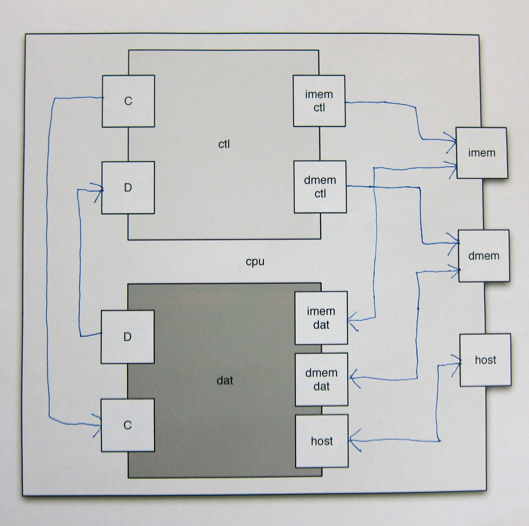
\includegraphics[width=0.9\textwidth]{../tutorial/figs/cpu.png} 
\end{center}

\end{columns}
\end{frame}

\begin{frame}[fragile]{Partial Interface Fulfillment}
\begin{columns}
\column{0.40\textwidth}

\begin{scala}
class Cpath extends Component {
  val io = new CpathIo();
  ...
  io.imem.isVal := ...;
  io.dmem.isVal := ...;
  io.dmem.isWr  := ...;
  ...
}

class Dpath extends Component {
  val io = new DpathIo();
  ...
  io.imem.raddr := ...;
  io.dmem.raddr := ...;
  io.dmem.wdata := ...;
  ...
}
\end{scala}

\column{0.50\textwidth}

\begin{center}
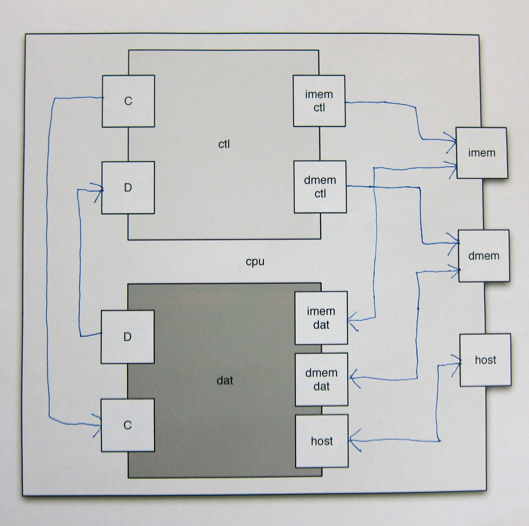
\includegraphics[width=0.9\textwidth]{../tutorial/figs/cpu.png} 
\end{center}

\end{columns}
\end{frame}

\begin{frame}[fragile]{Multiple Partial Bulk Connections}
\begin{columns}
\column{0.40\textwidth}

\begin{scala}
class Cpu extends Component {
  val io = new CpuIo()
  val c  = new CtlPath()
  val d  = new DatPath()
  c.io.ctl  <> d.io.ctl
  c.io.dat  <> d.io.dat
  c.io.imem <> io.imem
  d.io.imem <> io.imem
  c.io.dmem <> io.dmem
  d.io.dmem <> io.dmem
  d.io.host <> io.host
}
\end{scala}

\column{0.50\textwidth}

\begin{center}
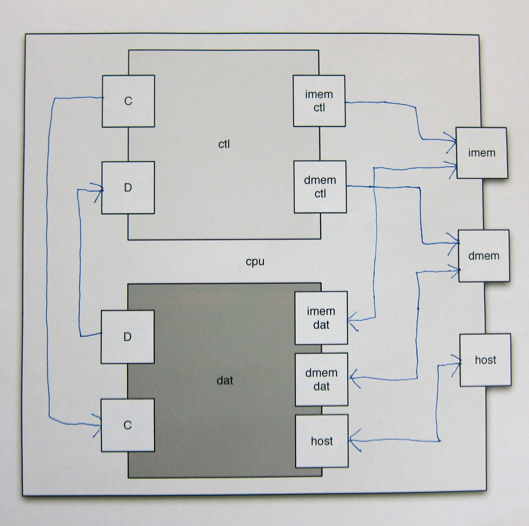
\includegraphics[width=0.9\textwidth]{../tutorial/figs/cpu.png} 
\end{center}

\end{columns}
\end{frame}

\begin{frame}
\begin{columns}

\column{0.65\textwidth}

\frametitle{Resources}
\begin{itemize}
\item Scala books
\item \url{chisel.eecs.berkeley.edu}
\item Chisel writings
\begin{itemize}
\item Chisel tutorial
\item Chisel manual
\item Chisel DAC-2012 paper
\end{itemize}
\item Chisel examples on github
\begin{itemize}
\item Sodor Processors
\item Floating Point Unit
\item Rocket Processor
\item Hwacha Vector Unit
\end{itemize}
\end{itemize}

\column{0.25\textwidth}

\begin{center}

\includegraphics[height=0.4\textheight]{../bootcamp/figs/programming-scala.pdf} \\
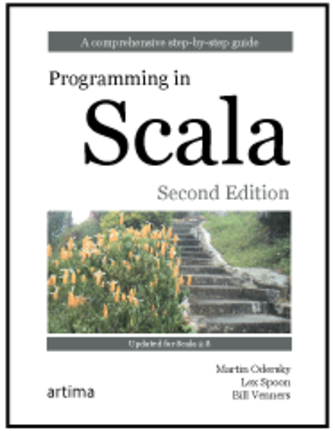
\includegraphics[height=0.4\textheight]{../bootcamp/figs/programming-in-scala.pdf}
\end{center}

\end{columns}
\end{frame}

\begin{frame}
\frametitle{Advanced Topics}
\begin{itemize}
\item Functional Composition
\item Object Oriented Interfaces
\item Layering Domain Specific Languages on Top
\end{itemize}
\end{frame}

\begin{frame}[fragile]{Functional Composition}
\begin{columns}

\column{0.45\textwidth}
\verb+Map(ins, x => x * y)+ \\
\begin{center}
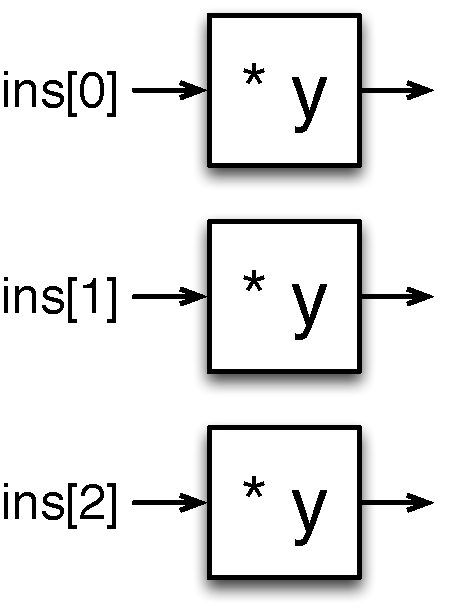
\includegraphics[height=0.6\textheight]{../bootcamp/figs/map.pdf} \\[2cm]
\end{center}

\column{0.45\textwidth}
\vskip2mm
\verb+Chain(n, in, x => f(x))+ \\
\begin{center}
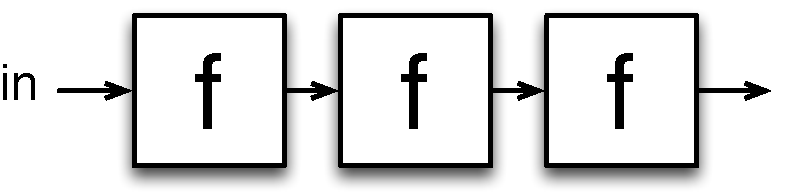
\includegraphics[width=0.9\textwidth]{../bootcamp/figs/chain.pdf} \\
\end{center}

\verb+Reduce(data, Max)+ \\
\begin{center}
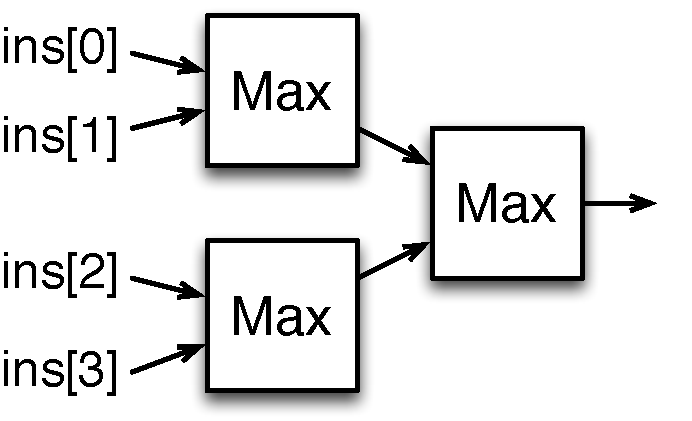
\includegraphics[width=0.9\textwidth]{../bootcamp/figs/reduce.pdf} \\
\end{center}

\end{columns}
\end{frame}

\begin{frame}[fragile]{Object-Oriented Parameterized Interfaces}
\begin{scala}
class Router extends Component {
  val depth = 32
  val n     = 4
  val io    = new RouterIO(n)
  val tbl   = Mem(depth){ UFix(width = sizeof(n)) }
  
  ...
}
\end{scala}
\begin{center}
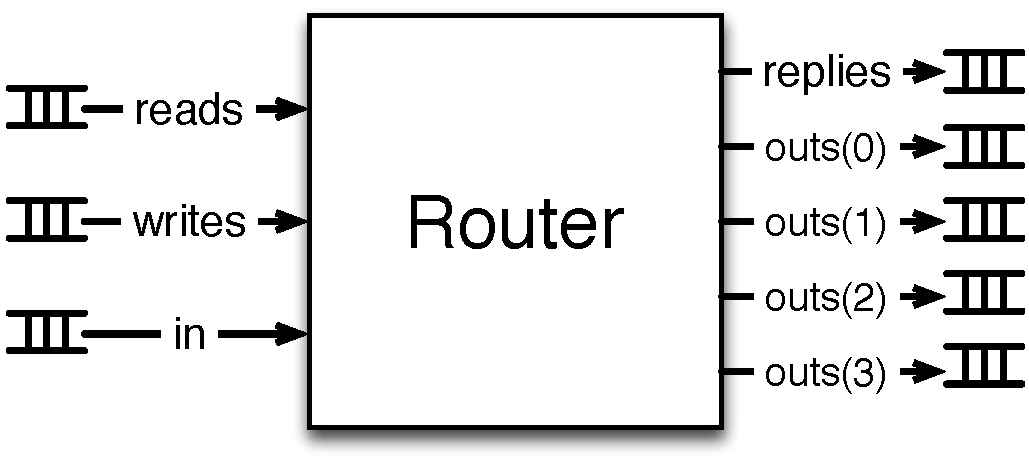
\includegraphics[height=0.45\textheight]{../bootcamp/figs/trouter.pdf} 
\end{center}
\end{frame}

\begin{frame}[fragile]{Router Interface}
\begin{scala}
class RouterIO(n: Int) extends Bundle {
  override def clone = new RouterIO(n).asInstanceOf[this.type]
  val reads   = new DeqIO(){ new ReadCmd() }
  val replies = new EnqIO(){ UFix(width = 8) }
  val writes  = new DeqIO(){ new WriteCmd() }
  val in      = new DeqIO(){ new Packet() }
  val outs    = Vec(n){ new EnqIO(){ new Packet() } }
}
\end{scala}
\begin{center}
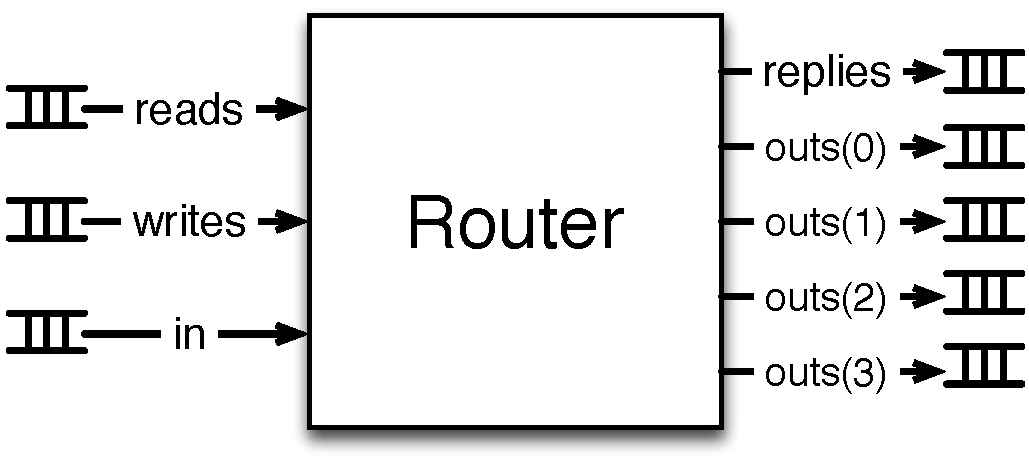
\includegraphics[height=0.45\textheight]{../bootcamp/figs/trouter.pdf} 
\end{center}
\end{frame}

\begin{frame}[fragile]{Complete Router Interface}

{\lstset{basicstyle={\scriptsize\ttfamily}}
\begin{scala}
class ReadCmd extends Bundle {
  val addr = UFix(width = 32)
}

class WriteCmd extends ReadCmd {
  val data = UFix(width = 32)
}

class Packet extends Bundle {
  val header = UFix(width = 8)
  val body   = Bits(width = 64)
}

class RouterIO(n: Int) extends Bundle {
  override def clone = new RouterIO(n).asInstanceOf[this.type]
  val reads   = new DeqIO(){ new ReadCmd() }
  val replies = new EnqIO(){ UFix(width = 8) }
  val writes  = new DeqIO(){ new WriteCmd() }
  val in      = new DeqIO(){ new Packet() }
  val outs    = Vec(n){ new EnqIO(){ new Packet() } }
}
\end{scala}
}
\end{frame}

\begin{frame}[fragile]{Router Guts}

{\lstset{basicstyle={\scriptsize\ttfamily}}
\begin{scala}
class RouterIO(n: Int) extends Bundle {
  override def clone = new RouterIO(n).asInstanceOf[this.type]
  val reads   = new DeqIO(){ new ReadCmd() }
  val replies = new EnqIO(){ UFix(width = 8) }
  val writes  = new DeqIO(){ new WriteCmd() }
  val in      = new DeqIO(){ new Packet() }
  val outs    = Vec(n){ new EnqIO(){ new Packet() } }
}

class Router extends Component {
  val depth = 32
  val n     = 4
  val io    = new RouterIO(n)
  val tbl   = Mem(depth){ UFix(width = sizeof(n)) }
  
  when(io.reads.valid && io.replies.ready) { 
    val cmd = io.reads.deq();  io.replies.enq(tbl(cmd.addr))  
  } .elsewhen(io.writes.valid) { 
    val cmd = io.writes.deq(); tbl(cmd.addr) := cmd.data
  } .elsewhen(io.in.valid) {
    val pkt = io.in.deq(); io.outs(tbl(pkt.header(0))).enq(pkt) 
  } 
}
\end{scala}
}
\end{frame}

\begin{frame}[fragile]{Object Oriented FIFOIO}

{\lstset{basicstyle={\scriptsize\ttfamily}}
\begin{scala}
class EnqIO[T <: Data]()(data: => T) extends FIFOIO()(data) {
  def enq(dat: T): T = { valid := Bool(true); data := dat; dat }
  valid := Bool(false)
  for (io <- data.flatten.map(x => x._2))
    io := UFix(0, io.getWidth())
}

class DeqIO[T <: Data]()(data: => T) extends FIFOIO()(data) {
  flip()
  ready := Bool(false)
  def deq(b: Boolean = false): T = { ready := Bool(true); data }
}

class Filter[T <: Data]()(data: => T) extends Component {
  val io = new Bundle {
    val in  = new DeqIO(){ data }
    val out = new EnqIO(){ data }
  }
  when (io.in.valid && io.out.ready) {
    io.out.enq(io.in.deq())
  }
}
\end{scala}
}
\end{frame}



\end{document}
